\setstretch{1.6}
\sectiontitle{6}{Path Planning Integration}
\lhead{Path Planning Integration} % section header
Prior to the start of this thesis a path planning algorithm had been developed specifically for this system by another student. However that algorithm was in matlab and had not been incorporated into the code base. It was therefore a necessary step to determine how this pathplanning should be incorporated into the system in order to allow path following. This brief section outlines the methodology and implementation of the path planning integration.

\subsection{Description of the Path Planning Algorithm}
The algorithm generates paths by combining geometric primitives, specifically constant curvature arcs and straight-line segments. The generated path is composed of piecewise constant curvature segments, with a non-differentiable curvature profile over time. To construct efficient and safe trajectories, the algorithm uses a look-ahead strategy combined with dynamic programming. At each step, it evaluates multiple motion primitives to connect the current waypoint to the next, considering how different curvature transitions affect the downstream trajectory. The selection aims to minimize the total path length and the number of curvature changes (which relate to crack generation in the tissue). This eventually outputs a list of straight line segments and curvature segments that create a continuous path. For more details on the algorithm see the final report of Charles Hong in appendix D.

\subsection{Methods}
Several strategies for incorporating the MATLAB-based path planning algorithm into the control system were considered. One option was to rewrite the algorithm in C++ and embed it directly into the codebase. However, since the planner is intended for precomputed paths rather than real-time operation, this approach was deemed unnecessary and inefficient.
\newline \newline
Instead, a more modular approach was adopted: the system codebase was adapted to read a simple CSV file containing path segments defined by arc length and curvature, a file that is generated by the MATLAB path planning algorithm. A dedicated module, \texttt{PathProcessing}, was implemented to parse this file and interpolate a continuous trajectory. 

\subsection{Implementation}
The \texttt{PathProcessing} module was implemented to parse the file generated by the pathplanning algorithm. The module imports and interpolates the data from the file containing segment lengths and curvatures. After parsing the file, it stores the values for use in feedforward control and trajectory generation.
\newline \newline
To generate a continuous path, each segment is discretized into steps of length \( \Delta l \), and waypoints are computed based on whether the segment is straight or curved. The path starts at \( (x_0, z_0) = (0, 0) \) with an initial heading \( \gamma = -\frac{\pi}{2} \).

For \textbf{straight segments} (\( |\kappa| < 10^{-6} \)), the position is updated using:
\begin{align}
x_{i+1} &= x_i + \Delta l \cdot \cos(\gamma) \\
z_{i+1} &= z_i - \Delta l \cdot \sin(\gamma)
\end{align}

For \textbf{curved segments} (\( |\kappa| \geq 10^{-6} \)), the radius \( R = \frac{1}{\kappa} \) is used to compute:
\begin{align}
\Delta \gamma &= \Delta l \cdot \kappa \\
x_{i+1} &= x_i + R \left( \sin(\gamma + \Delta \gamma) - \sin(\gamma) \right) \\
z_{i+1} &= z_i + R \left( \cos(\gamma + \Delta \gamma) - \cos(\gamma) \right) \\
\gamma &\leftarrow \gamma + \Delta \gamma
\end{align}

An optional positional offset can also be applied to the generated waypoints to shift the path to the starting point of where the ribbon enters the medium. The resulting list of points. along with curcature information at each step is stored and made available to path following modules. 

\subsection{Results}
\begin{figure}[htbp]
    \centering
    \begin{subcaptionbox}{Picture of ribbon in agarose annotated with tip and pre-tip detections\label{fig:left}}[0.45\linewidth]
        {\includegraphics[width=\linewidth]{}}
    \end{subcaptionbox}
    \hspace{0.05\linewidth}
    \begin{subcaptionbox}{Picture of ribbon in vobine gelatin\label{fig:right}}[0.45\linewidth]
        {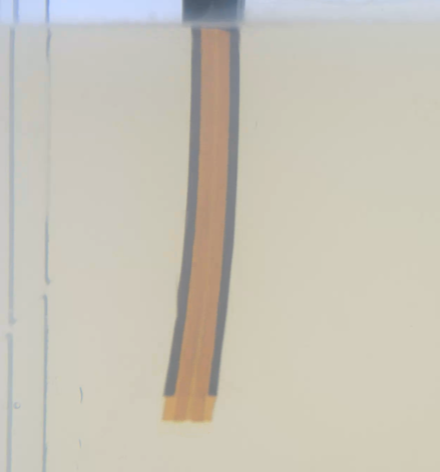
\includegraphics[width=\linewidth]{images/RibbonPicture/gelatin2.PNG}}
    \end{subcaptionbox}
    \caption{Pictures of the ribbon being inserted into an agarose brain phanton (a) vs a bovine gelatin brain phantom (b)}
    \label{fig:side_by_side}
\end{figure}

\subsection{Discussion}

This approach simplifies the integration while keeping the control framework flexible and decoupled from the planning logic.

This modular implementation ensures that path planning remains decoupled from the runtime control logic while providing the necessary trajectory resolution and curvature profile for smooth control.

Future path should have continuous change of curvature